% Préambule APMEP - Annales
% Auteurs
% tapuscrit : Hubert Proton
% relecture : Mathieu Drillet et Michel Suquet
% chiffres TikZ : Hubert Proton
% chiffres pstricks :
% modifications : v3 : changement d'une figure
% Remerciements :
% version 3 : 2026-07-05
%
\documentclass[12pt,a4paper,french]{article}

% des paquets
%%% codage et police utilisée
\usepackage[T1]{fontenc}
\RequirePackage{iftex}
\iftutex % moteur utf-8 lualatex, xelatex
	\usepackage{fourier-otf} % remplace fourier pour moteur utf8 (LuaLaTeX, XeLaTeX)
	% Alternatives nécéssites (LuaLaTeX, XeLaTeX)
    \usepackage{hyperref}
	%\usepackage{fontspec}% pour utiliser les polices système
\else % pour les autres moteurs latex, pdflatex
	\usepackage[utf8]{inputenc}
	\usepackage{fourier}
	\usepackage{amsmath,amssymb}
    \usepackage[dvips]{hyperref}
    \renewcommand{\ttdefault}{lmtt}
\fi
\usepackage[normalem]{ulem}
\usepackage{pifont}
\usepackage{lscape}
% tableaux
\usepackage{multicol}
\usepackage{multirow}
\usepackage{tabularx}
\usepackage{tabularray}
% texte et composition
\usepackage{textcomp}
\usepackage{babel}
\usepackage[np]{numprint}
%
\usepackage{fancyhdr}
\usepackage{makeidx}
\makeindex
% pour le symbole \euro{}
\usepackage{eurosym}
\DeclareRobustCommand{\officialeuro}{%
  \ifmmode\expandafter\text\fi
  {\fontencoding{U}\fontfamily{eurosym}\selectfont e}}
\AtBeginDocument{\renewcommand{\euro}{\officialeuro}}
% couleurs étendues
\usepackage{xcolor}
% pour les listes
\usepackage{enumitem}
% Enumérations réglées par défaut
\setlist[itemize]{label=\textbullet,leftmargin=5mm,labelwidth=3mm,labelsep=2mm,align=left}
\setlist[enumerate]{labelindent=0pt, leftmargin=5mm, labelsep=2mm, labelwidth=3mm,labelsep=2mm, align= left}
\setlist[enumerate,1]{label = \textbf{\arabic*.}}
\setlist[enumerate,2]{label = \textbf{\alph*.}}
\setlist[enumerate,3]{label = \textbf{\roman*.}}
% pour l'ajustement des boîtes (chiffres…)
\usepackage{adjustbox}
% pour ne pas commencer un exercice en fin de page
\usepackage{needspace}
%
% Taille de la zone d'écriture
\usepackage[left=1.5cm,right=1.5cm,top=3cm,bottom=3cm]{geometry}
\setlength{\headheight}{15pt}
\setlength{\parindent}{0mm}
%
Formatage du PDF
\hypersetup{%
    auteur du PDF = {APMEP},
    pdfsubject = {Troisième, Série générale},
    pdftitle = {Brevet des collèges -- Session 2026},
    allbordercolors = blanc,
    pdfstartview=FitH
}
% Pour scratch (code)
\usepackage{scratch3}
% Pour le code Python
\usepackage{listings}
\lstdefinestyle{python}{
  langue=Python,
  style de base=\ttfamily\small,
  style_mot_clé=\color{bleu}\bfseries,
  style de commentaire=\color{gris}\itshape,
  style de chaîne=\color{orange},
  nombres=gauche,
  style_numéro=\tiny\color{gris},
  breaklines=true,
  cadre=unique,
  couleur de fond=\color{gris!5},
  taille de l'onglet=4
}
  % d'utilisation (exemple)
  %\begin{lstlisting}[style=python]
%def seuil():
% n = 1
% p = 0,5
% tant que p < 0,6 :
% n = n + 1
% p = p*7/15 + 1/3
% retour n
%\end{lstlisting}


% Pour une visualisation de type tableau
\usepackage{pas-tableur}
%
%% pour PsTricks
\usepackage{pst-bezier}%% AVANT les autres PST
\usepackage{pstricks-add}
\usepackage{pst-func,pst-tree,pst-circ}
\usepackage{pst-eucl}
%% pour TikZ
\usepackage{tikz,pgfplots,pgf,tkz-tab,tikzpagenodes}
\usetikzlibrary{calc,patterns,decorations,arrows.meta,patterns.meta,arrows}
\pgfplotsset{compat=1.18,/pgf/number format/.cd,use comma}
\usepackage{icomma} % gestion des espaces autour des virgules
\DeclareMathSymbol{;}{\mathbin}{operators}{"3B}% pour un espacement correct du ; en mode maths
%%%%%%%%%%%%%%%%%%%%%%%%%%%%%%%%%%%%%%%%%%
% Définitions
%
% notation en mode mathématique et hors mode mathématique
\newcommand{\R}{\ensuremath{\mathbb{R}}}
\newcommand{\N}{\ensuremath{\mathbb{N}}}
\newcommand{\D}{\ensuremath{\mathbb{D}}}
\newcommand{\Z}{\ensuremath{\mathbb{Z}}}
\newcommand{\Q}{\ensuremath{\mathbb{Q}}}
\newcommand{\C}{\ensuremath{\mathbb{C}}}
%
\providecommand{\up}{\textsuperscript}
%
\newcommand{\vect}[1]{\overrightarrow{\,\mathstrut#1\,}}
\newcommand{\vectt}[1]{\overrightarrow{\,\mathstrut\text{#1}\,}}
%
\def\Oij{$\left(\text{O};\vect{\imath},\vect{\jmath}\right)$}
\def\Oijk{$\left(\text{O};\vect{\imath},\vect{\jmath},\vect{k}\right)$}
\def\Ouv{$\left(\text{O};\vect{u},\vect{v}\right)$}
%
\newcommand{\ds}{\displaystyle}
%
\renewcommand{\d}{\mathrm{\,d}}
\renewcommand{\i}{\mathrm{\,i\,}}
\newcommand{\e}{\mathrm{\,e\,}}
%%%%%%%%%%%%%%%%%%%%%%%%%%%%%%%%%%%%%%%%%%%


\begin{document}
%---------------------------------------------------------
% Réglage en tête, pied de page
%---------------------------------------------------------
\rhead{\textbf{A. P{}. ME P{}.}}
\lhead{\small Corrigé}
\lfoot{\small{Centres étrangers}}
\rfoot{\small{18 juin 2026}}
\pagestyle{fancy}
\thispagestyle{vide}

%---------------------------------------------------------
% Titre
%---------------------------------------------------------
\begin{center}
{\bfseries \Large
	\decofourleft~ Diplôme National du Brevet ~\decofourright\\[10pt]
	Série générale -- Centres étrangers -- 18 juin 2026
	\marginpar{\rotatebox{90}{\textbf{A. P{}. ME P{}.}}}\\[10pt]
	Corrigé}
\end{center}


\section*{\centering PREMIÈRE PARTIE : AUTOMATISMES (6 pts)}

\subsection*{Question 1}
	On range les valeurs dans l'ordre croissant : \np[°C]{-1}; \np[°C]{0} ; \np[°C]{1} ; \np[°C]{3} ; \np[°C]{7}.

	La médiane est la valeur qui est au milieu de la série, {c'est \np[°C]{1}.}

\subsection*{Question 2}
	\begin{minipage}[t]{0.4\linewidth}
		C'est le {motif n°8} qui est l'image du motif n°4 par cette traduction.
	\end{minipage}
	\hfill~
	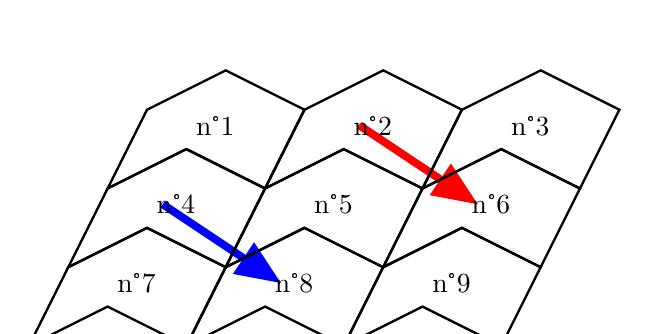
\begin{tikzpicture}[baseline={(current bounding box.center)}]
		\draw[->, >=triangle 45,line width=1mm, red](3.2,0.8)--(4.7,-0.2);
		\draw[->, >=triangle 45,line width=1mm, blue](0.7,-0.2)--(2.2,-1.2);
		\foreach \n/\x/\y in{1/0/0,2/2/0,3/4/0,4/-0.5/-1,5/1.5/-1,6/3.5/-1,7/-1/-2,8/1/-2,9/3/-2}{\begin{scope}[shift={(\x,\y)},rotate=0]
				\draw[line width=0.3mm](0,0)--(1,0.5)--(2,0)--(2.5,1)--(1.5,1.5)--(0.5,1)--cycle;\draw(1,0.8)node[right]{n°\n};
		\end{scope}}
	\end{tikzpicture}\hfill~

\subsection*{Question 3}
	Il y a 8 boules dont 3 sont rouges, donc {{$P(\text{rouge})=\dfrac38=\np{0.375}$}}

	\begin{minipage}{0,45\linewidth}
\subsection*{Question 4}
	On utilise la formule informée par c\oe{}ur \textbf{CAH}.

	{$\cos\left(\widehat{\text{LKJ}}\right)=\dfrac{\text{adjacent}}{\text{hypoténuse}}=\dfrac{\text{LK}}{\text{JK}}$}
	\end{minipage}
	\hfill~
	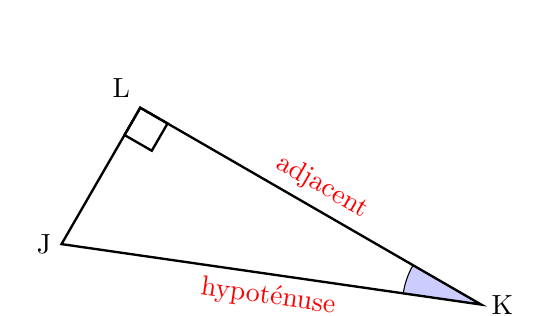
\begin{tikzpicture}[rotate=-30,baseline={(current bounding box.center)}]
		\draw[line width=0.3mm](0,0)rectangle(0.4,-0.4);
		\draw[fill=blue!20](5,0)--(4,0)arc(180:201.8:1)--cycle;
		\draw[line width=0.3mm](0,0)node[above left]{L}--(5,0)node[right]{K}node[midway, above, rotate=-30]{\textcolor{red}{adjacent}}--(0,-2)node[left]{J}node[midway, below, rotate=-8.2]{\textcolor{red}{hypoténuse}}--cycle;
	\end{tikzpicture}
	\hfill~

\subsection*{Question 5}
	{$\np{311200000}=\np{3.112}\times\np{100000000}$} \quad et \quad {$\np{100000000}=10^8$} (zérohuits),

	donc l'écriture scientifique de \np{311200000} est {$\np{3.112}\times10^8$}

\subsection*{Question 6}
	2~h~30~min c'est 2 heures plus la moitié d'une heure.

	Charlie a donc parcouru deux fois 40~km plus la moitié de 40~km :
	$40 \times 2 + 40 \div 2 = 80 + 20 = 100$.

	Au total, {Charlie a fait 100~km.}

\subsection*{Question 7}
	{$5(x+1)=5\times x + 5\times 1 = 5x+5$}, donc la forme factorisée est {{$5(x+1)$}.}

\subsection*{Question 8}
	La diminution du prix est calculée par \quad
	\begin{tabular}{c|c|c}
		                & en \euro{} & en \% \\ \hline
		    baisse & $x$ & 10 \\ \hline
		valeur initiale & 80 & 100
	\end{tabular}

	{$x=80\times\dfrac{10}{100}$}, qu'il faut retrancher du prix initial, donc le calcul à effectuer est { {$80-\dfrac{10}{100}\times80$}.}

\subsection*{Question 9}
\begin{center}
	\begin{tikzpicture}%compilateur avec pgfplots
	\begin{axis}[/pgf/number format/.cd, utilisez une virgule,
		style du titre = {alignement = centre},
		title={Hauteur d'eau dans le port de Quiberon -- 23 juillet 2025},
		xlabel={Heure (en h)},
		style xlabel={
			à={(étiquette de graduation cs:1)},
			ancre=nord-est},
		ylabel={Hauteur d'eau (en m)},
		x={13,6 mm}, y={13,6 mm},
		xmin = 12,5, xmax = 20,
		ymin = 2, ymax = 5,
		xtick = {13,14,15,16,17,18,19,20},
		xticklabels = {13~h, 14~h, 15~h, 16~h, 17~h, 18~h, 19~h, 20~h},
		distance ytick=1,
		style d'étiquette de coche={font=\footnotesize},
		numéro de graduation mineure = 1,
		grille=les deux]
		\addplot [line width=1.2pt,color=red,smooth,samples=100,domain= 17:20 ]{2.6 + 2.25*cos((x-17)*25.5)};
		\addplot [line width=1.2pt,color=red,smooth,samples=100,domain= 13:17 ]{2.4 + 2.45*cos((x-17)*20)};
		\draw[teal,line width=2pt] (axis cs: 14.5,4)node[below right]{env. 14 h 30}--(axis cs: 19,4)node[below left] {env 19 h};
	\end{axis}
\end{tikzpicture}
\end{center}
	Entre 14~h~30 à 19~h environ, le niveau a été plus élevé que 4~m, cela a donc duré {environ 4~h~30~min.}

\needspace{10\baselineskip}

\section*{\centering DEUXIÈME PARTIE (14 pts)}

\section*{Exercice 1 (4 points)}

\begin{énumérer}
	\item \hfill~\begin{tikzpicture}[baseline=(N.base)]
	\draw[->](0,0)node[below]{A}--(6.4,0)node[below]{B}--(9.6,0)node[below]{M};
	\draw[->](6,.4)rectangle(6.4,0)--(6.4,4.8) (9.2,0.4)rectangle(9.6,0)--(9.6,7.2);
	\draw[->][dashed](6.4,4.8)--(6.4,6)(9.6,7.2)--(9.6,8);
	\draw[->][dashed](8,0)arc(0:45:8);
	\draw[->](6.4,4.8)node[above right]{C};
	\draw[->,dashed](-0.5,-0.375)--(10,7.5);
	\draw[->](0,0)--(9.6,7.2)node[above](N){N};
	\end{tikzpicture}\hfill~

	Commencer par tracer le segment [AM] (\np[cm]{9.6}) avec le point B intercalé à \np[cm]{6.4} de A.

	Puis tracer les deux perpendiculaires en B et M.

	Laisser apparent un bel arc de cercle centré sur A et de rayon 8.

	À l'intersection avec la perpendiculaire en B, à la place du point C.

	On peut ensuite tracer la droite (AC) et placer N à l'intersection avec la perpendiculaire en M.

	\item ABC est un triangle rectangle en B, selon le théorème de Pythagore, {$\text{AC}^2=\text{AB}^2+\text{BC}^2$}.

	Donc {$\text{BC}^2=8^2-\np{6.4}^2=\np{23.04}$} et {$\text{BC}=\sqrt{\np{23.04}}=\np{4.8}$}.

	La longueur BC mesure \np[cm]{4.8}.

	\item (BC) et (MN) sont toutes deux perpendiculaires à (AM).

	Comme deux droites perpendiculaires à une même troisième droite sont parallèles entre elles, (BC) et (MN) sont parallèles.

	\item \begin{itemize}
		\item Les points A, B et M sont alignés;
		\item les points A, C et N sont alignés;
		\item (BC) et (MN) sont parallèles.
	\end{itemize}
	Donc, selon le théorème de Thalès, \quad {$\dfrac{\text{AB}}{\text{AM}}=\dfrac{\text{AC}}{\text{AN}}=\dfrac{\text{BC}}{\text{MN}}$}

	On peut donc calculer : \quad
	{$\text{MN}=\dfrac{\text{BC}\times\text{AM}}{\text{AB}}=\np{7.2}$}\quad et \quad
	{$\text{AN}=\dfrac{\text{AC}\times\text{AM}}{\text{AB}}=\np{12}$}.

	Les longueurs MN et AN sont respectivement \np[cm]{7.2} et \np[cm]{12}.

	\item Le périmètre du triangle ABC est de {$\np{6.4}+\np{4.8}+8=\np[cm]{19.2}$}.

	Comme A, C et N sont alignés, {$\text{CN}=\np[cm]{4}$}.

	Donc le périmètre de BMNC est égal à {$\np{3.2}+\np{7.2}+\np{4}+\np{4.8}=\np[cm]{19.2}$}.

	Les deux figures ont le même périmètre et celui-ci est de \np[cm]{19.2}.
\end{énumérer}

\needspace{10\baselineskip}

\section*{Exercice 2 (\np{3,5} points)}
\subsection*{Partie A}
\begin{énumérer}
	\item La longueur totale d'un bonbon est de \np[mm]{15}.

	À chaque extrémité, il y a une demi-boule de rayonne \np[mm]{2.5}.

	Donc la partie cylindrique a une hauteur égale à {$15-2\times\np{2.5}=\np[mm]{10}$.}

	\item \begin{énumérer}
		\item La partie cylindrique a pour base un disque de rayonne \np[mm]{2.5},

		son aire est égale à {$\pi \times\np{2.5}^2\approx\np[mm^2]{19.63}$}.

		La hauteur du cylindre est de \np[mm]{10},

		donc son volume est égal à {$10\times(\pi\times\np{2.5}^2)\approx \np[mm^3]{196}$.}

		\item Les deux demi-boules qui constituent les extrémités ont, ensemble, le volume d'une boule de rayon \np{2.5}, soit \quad {$\dfrac43 \times \pi\times \np{2.5}^3\approx \np[mm^3]{65.4}$}.

		Léa a donc raison, puisque la somme des volumes de la partie cylindrique et des deux extrémités est égale à {$\np{196.3}+\np{65.4}=\np{261.7}$} qui s'arrondit à \np[mm^3]{262}.

		\textit{Variante:} Le volume des deux demi-boules est environ \np[mm^3]{65}, le volume total d'un bonbon est de \np[mm^3]{261}, donc Léa a raison.
	\end{énumérer}

	\item Un bonbon demande un volume d'environ \np[mm^3]{262},

	donc pour produire \np{300000} bonbons, il faut {$\np{300000}\times262=\np[mm^3]{78600000}$} de mélange.

	Ou \quad {$\np[litre]{1} = \np[dm^3]{1} = \np[cm^3]{1000} = \np[mm^3]{1000000}$}.

	Donc \quad {$\np[mm^3]{78600000}=\np[litres]{78.6}$} :

	83~litres seront donc plus que suffisants pour produire \np{300000}~bonbons.
\end{énumérer}

\subsection*{Partie B}

	Avec le format A, Léa paiera {$2\times\np{7.90}=\np[\euro{}]{15.80}$} pour 1 kilo de bonbons.

	Avec le format B, il lui faudra acheter 4 sachets, les 3 premiers à \np[\euro{}]{4.30}, le quatrième à \np[\euro{}]{2.15}.

	Cela lui coûtera au total \quad {$3\times\np{4.30}+\np{2.15}=\np[\euro{}]{15.05}$}.

	Léa a donc intérêt à profiter de la promotion sur les sachets B.

\needspace{10\baselineskip}
\section*{Exercice 3 (\np{4,5} points)}
\begin{énumérer}
	\item On choisit $1$ comme nombre de départ :\qquad
	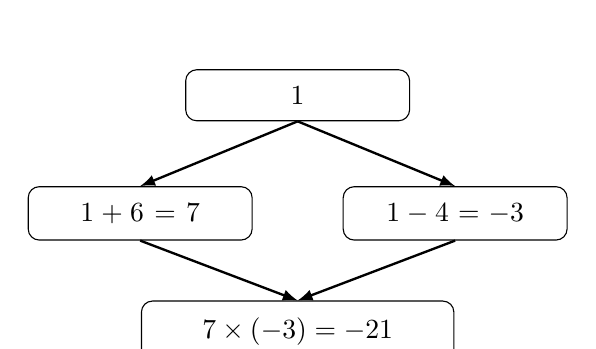
\begin{tikzpicture}[every node/.style={align=center,inner ysep=6pt,inner xsep=12pt,minimum width=2cm, rounded corners}, baseline={(a.base)}]
	\node(a)at(0,0)[text width=2cm,draw]{1};
	\node(b)at(-2,-1.5)[text width=2cm,draw]{{$1+6=7$}};
	\node(c)at(2,-1.5)[text width=2cm,draw]{{$1-4=-3$}};
	\node(d)at(0,-3)[draw]{\quad$7\times(-3)=-21$\quad};
	\draw[->,>=latex,line width=0.3mm](a.south)--(b.north);
	\draw[->,>=latex,line width=0.3mm](a.south)--(c.north);
	\draw[->,>=latex,line width=0.3mm](b.south)--(d.north);
	\draw[->,>=latex,line width=0.3mm](c.south)--(d.north); \end{tikzpicture}

	Si on choisit $1$, on obtient effectivement $-21$ avec le programme A.

	\item {$10\xrightarrow{\text{élever au carré}}10^2=100$\quad puis \quad $100 \xrightarrow{\text{soustraire }9}100-9=91$}

	Avec le programme B, on obtient 91$ lorsque le nombre de départ est 10$.

	\item Si on choisit $x$ comme nombre de départ, le programme B calcule {$x^2-9$}.

	On cherche donc pour quelle(s) valeur(s) de $x$ onobtient $16$,

	autrement dit \quad {$x^2-9=16\iff x^2-25=0$}.

	On remarque que {$25=5^2$}, donc on peut factoriser une identité remarquable et l'équation à résoudre devient {$(x-5)(x+5)=0$.}

	Un produit est nul si et seulement si un des facteurs est nul; il y a donc deux solutions qui sont $-5$ et $5$.

	Si on choisit un de ces deux nombres, on obtient 16$ avec le programme B.

	\item \begin{minipage}[t]{0.45\linewidth} Ligne 3, on ajoute 6, ligne 4, on soustrait 4 et enfin ligne 5 on fait le produit des 2 résultats intermédiaires.
	\end{minipage}\hfill~
	\begin{scratch}[num blocks,num start=3, baseline=3]
	\blockvariable{mettre \selectmenu{Valeur 1} à {\ovaloperator{\ovalsensing{réponse} + \ovalnum{6}}}}
	\blockvariable{mettre \selectmenu{~Valeur 2} à {\ovaloperator{\ovalsensing{réponse} - \ovalnum{4}}}}
	\blockvariable{mettre \selectmenu{Résultat} à \ovaloperator{\ovalvariable{Valeur 1} ~* \ovalvariable{Valeur 2}}}
	\end{scratch}\hfill~
	\item On choisit $x$ comme nombre de départ dans le programme A :

	\begin{center}
		\begin{tikzpicture}[every node/.style={align=center,inner ysep=6pt,inner xsep=12pt,minimum width=2cm, rounded corners}, baseline={(a.base)}]
	\node(a)at(0,0)[dessiner]{$x$};
	\node(b)at(-2,-1.5)[draw]{{$x+6$}};
	\node(c)at(2,-1.5)[draw]{{$x-4$}};
	\node(d)at(0,-3)[draw]{$(x+6)(x-4)$};
	\draw[->,>=latex,line width=0.3mm](a.south)--(b.north);
	\draw[->,>=latex,line width=0.3mm](a.south)--(c.north);
	\draw[->,>=latex,line width=0.3mm](b.south)--(d.north);
	\draw[->,>=latex,line width=0.3mm](c.south)--(d.north); \end{tikzpicture}
	\end{center}

	On développe : \quad {$(x+6)(x-4)=x^2-4x+6x-24=x^2+2x-24$}.

	Avec le programme A, on calcule {$x^2+2x-24$}.

	\item On sait que le programme A calcule \quad {$x^2+2x-24$} \quad et le programme B \quad {$x^2-9$}.

	Les deux programmes donnent le même résultat si et seulement si \quad {$x^2+2x-24=x^2-9$}.

	Cette équation peut se simplifier en soustrayant $x^2$ à chaque membre, et elle devient :

	$\begin{aligned}
			2x-24=-9&\iff2x=15\\&\iff x=\dfrac{15}{2}
		\end{aligned}$

	Les deux programmes donnent le même résultat si on choisit comme nombre de départ {$\dfrac{15}{2}=\np{7.5}$} et ce résultat est \np{47.25}.
\end{énumérer}
\end{document}